Lors de tout mes tests sur la carte de développement, j'ai utilisé l'outil \textit{rtspin} de \textit{liblitmus} afin de générer des tâches temps réel. Cet outil permet de générer des tâches avec des paramètres spécifiques, comme le pire temps d'exécution, la période, le processeur sur lequel la tâche doit s'exécuter, etc. Cependant, il ne permet pas de générer des tâches ayant des temps d'exécution différents sur différents processeurs. Cela est un problème, car cela ne permet pas de mettre en valeur la nature hétérogène de la plateforme sur laquelle nous travaillons. C'est pourquoi je me suis intéressé durant une partie de mon stage à créer de telles tâches.

\subsection{Mesure de temps d'exécution}
Il est important de pouvoir mesurer de manière suffisamment précise le temps d'exécution d'une tâche. Pour cela, ma première idée était d'utiliser le module \texttt{time} de Linux. Cependant, ce module ne permet pas de mesurer des temps d'exécution inférieurs à la milliseconde. Cela est dù au fait que le module \texttt{time} utilise le timer du noyau Linux qui a une précision de 1ms. Cela est bien trop imprécis pour mesurer des temps d'exécution de tâches temps réel. J'ai donc d'abord créé un script \texttt{bash} utilisant un autre temps Linux. Ce script est présent dans le listing \ref{annexe:precisiontime} et fut utilisé pour tous mes essais préliminaires. Cependant, ce script, malgré sa plus grande précision, mesurait toujours un temps minimum : environ 6ms. Je n'ai pas pu le montrer, mais ce temps semble venir du démarrage du script, puis du démarrage du programme appelé. Il a donc été utile pour comparer des tâches entre elles, mais n'était pas assez précis pour connaître le temps d'exécution d'une tâche.


\subsection{Génération de tâches répétables}
\label{section:generation-taches-repetables}

Mon objectif était alors de générer des tâches qui s'exécutent à des vitesses différentes sur les différents processeurs, tout en ayant un temps d'exécution qui ne varie qu'un minimum entre deux exécutions sur un même processeur.

\subsubsection{Première idée : \textit{checksum} d'un fichier}

Ma première idée était de calculer la checksum d'un fichier de petite taille. La taille du fichier permettrait alors de faire varier le temps d'exécution. Cette opération était principalement calculatoire, j'avais espoir que le temps d'exécution ne varie pas trop entre deux exécutions sur un même processeur. Cependant, cette opération semblait posséder trop d'accès à la mémoire et au stockage : deux choses que je ne voulais pas prendre en compte dans mon temps d'exécution. C'est ce que j'ai pu voir sur l'exécution d'une telle tâche, sur laquelle je réalise la \gls{checksum md5} sur un fichier de code de 95KiB, j'ai donc abandonné cette idée.

\subsubsection{Deuxièle idée : somme sur un grand nombre d'entiers}

Ma deuxième idée était de faire une somme sur un grand nombre d'entiers. Cette opération est aussi calculatoire, mais ne possède pas d'accès mémoire. J'ai donc créé un programme qui réalise une somme sur un grand nombre d'entiers. Ce programme est présent en annexe au listing \ref{annexe:sum-int}. Il contient aussi d'autres essais, et le choix de l'essai se fait lors de l'appel du programme. On notera par exemple que la variable sur laquelle on réalise la somme est déclarée en tant que \texttt{volatile} afin d'éviter que le compilateur optimise le code.

J'ai ensuite utilisé ce programme pour générer des tâches avec des temps d'exécution différents. Après beaucoup d'essais, et en désactivant les optimisations de compilation, j'ai réussi à obtenir des tâches avec des temps d'exécution différents. On peut alors voir le temps d'exécution en fonction de l'entier sur lequel on réalise la somme. J'ai ici réalisé le test sur deux processeurs : CPU0 qui est un processeur A53 et CPU5 qui est un des deux A72. On peut voir sur la figure \ref{fig:sum_int} que le temps d'exécution est bien différent entre les deux processeurs. Cependant, on peut voir que le temps d'exécution est légèrement variable sur un même processeur. Cela est dù au fait que le processeur est partagé entre plusieurs tâches, et que le temps d'exécution d'une tâche dépend de la charge du processeur. Cela est donc un problème pour mesurer le temps d'exécution d'une tâche. Cependant, cela ne pose pas de problème pour générer des tâches avec des temps d'exécution différents. En effet, si l'on prend un entier $n$ et que l'on réalise la somme sur les $n$ premiers entiers, on obtient un temps d'exécution différent pour chaque valeur de $n$. On peut donc générer des tâches avec des temps d'exécution différents en choisissant un entier $n$ différent pour chaque tâche. Cela est donc une solution pour générer des tâches avec des temps d'exécution différents sur différents processeurs.

\begin{figure}[H]
    \centering
    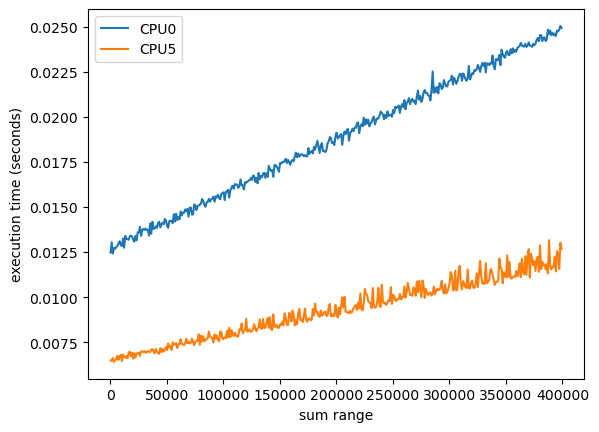
\includegraphics[width=0.9\textwidth]{Images/graphSum0and5.png}
    \caption{Temps d'exécution en fonction de l'entier sur lequel on réalise la somme}
    \label{fig:sum_int}    
\end{figure}


On remarque aussi que le temps d'exécution semble être linéaire avec l'entier sur lequel on réalise la somme. Il m'a alors été recommandé, lors d'un séminaire où j'ai pu présenter les travaux de mon stage au laboratoire, d'étudier si cette différence de temps d'exécution pouvait être corrélée avec les différentes fréquences des processeurs. En réutilisant les données qui ont permis de tracer le graphe de la figure \ref{fig:sum_int}, j'ai pu obtenir les régressions linéaires suivantes pour les deux processeurs :
% CPU0(n) =  3.0652132638329e-08 n +  0.012679295825389528
% CPU5(n) =  1.3932465779161102e-08 n +  0.006507234980479443

\begin{figure}[H]
    \centering
    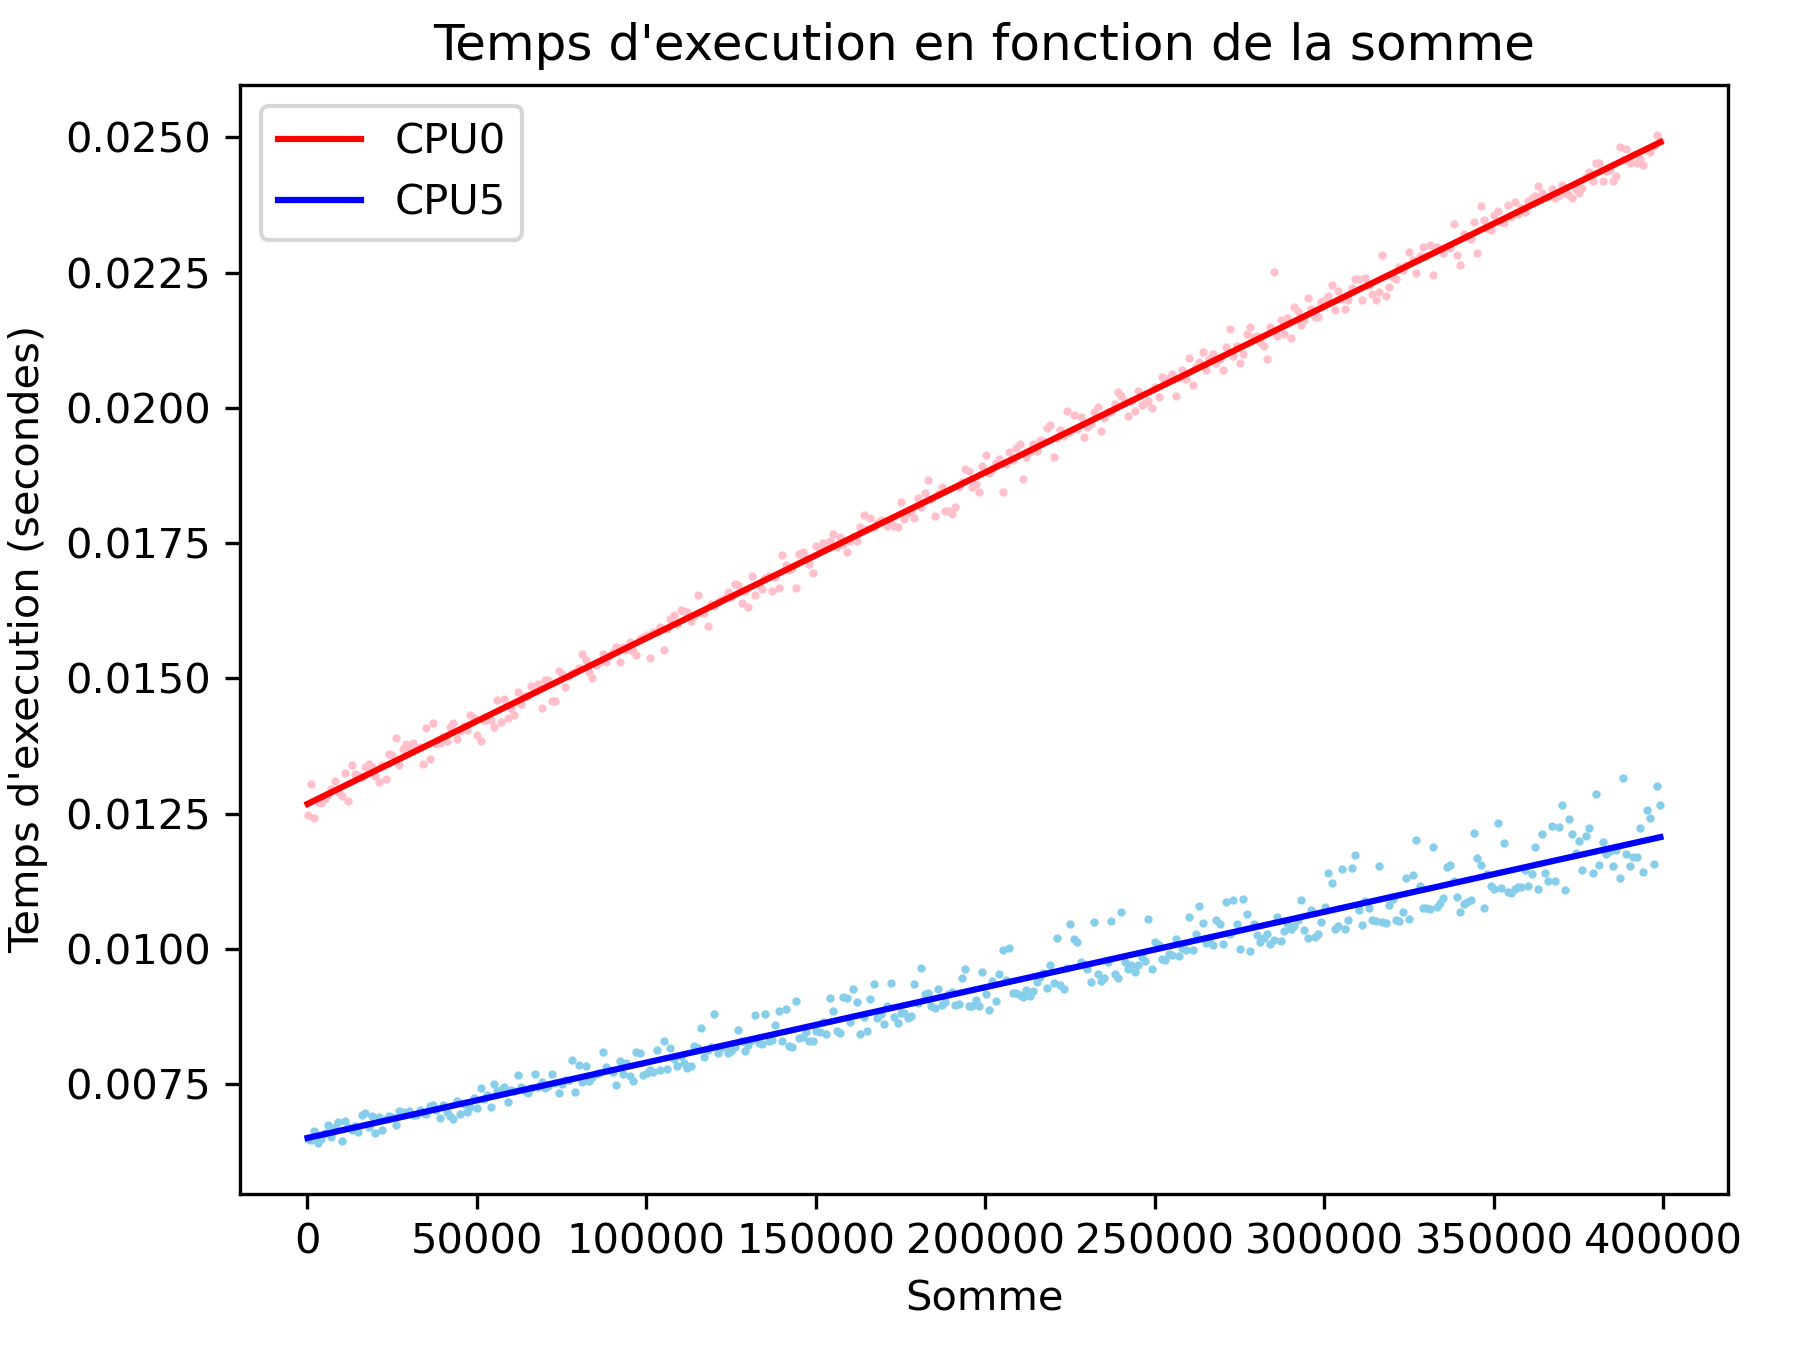
\includegraphics[width=0.9\textwidth]{Images/linear_regression.png}
    \caption{Régression linéaire du temps d'exécution en fonction de l'entier sur lequel on réalise la somme}
\end{figure}

On obtient alors les régressions linéaires suivantes à l'aide d'un script \texttt{python} :
\[
    CPU0(n) =  3.065 \times 10^{-8} n +  0.0127 
\] 
\[
    CPU5(n) =  1.393 \times 10^{-8} n +  0.0065
\]

Les processeurs A53 sont à une fréquence de 1.5GHz, et les A72 à une fréquence de 2GHz. On peut donc voir que la pente de la régression linéaire est plus grande pour les A53 que pour les A72. Cela est cohérent avec le fait que les A53 sont moins puissants que les A72. Cependant, on ne retrouve pas le rapport de puissance entre les deux processeurs. En effet $\frac{3.065}{1.393} = 2.200 \neq \frac{2}{1.5} = 1.333$ ce qui signifie que la différence de performance entre les deux processeurs n'est pas uniquement due à la différence de fréquence.


Cela semble être dù au fait que les processeurs A72 ont d'autres avantages comme :
\begin{itemize}
    \item Un parallélisme des instructions qu'il peut exécuter (\textit{3 way super scalar}) contrairement aux 2 instructions en parallèle des A53
    \item \textit{Out of order execution}, qui permet l’exécution dans le désordre de certaines instructions, ce qui permet de ne pas attendre qu'une instruction soit terminée pour en exécuter une autre
\end{itemize}

Ces deux avantages permettent aux A72 d'être plus performants que les A53, et donc d'avoir un temps d'exécution plus faible pour une même somme.

Je n'ai cependant pas eu le temps d'étudier cela plus en profondeur, par exemple, en mesurant le temps d'une manière à ne pas prendre en compte le démarrage des tâches. 


\subsubsection{Troisième idée : utilisation des instructions SIMD}

Une dernière idée proposée par Antoine \textsc{bertout} était l'utilisation des instructions SIMD. Ces instructions permettent de réaliser des opérations sur plusieurs entiers en même temps. Cela permet de réduire le temps d'exécution d'une opération. L'idée était alors d'utiliser ces instructions spécialisées, afin de mettre en valeur la différence de performance entre les deux processeurs. En effet, on s'attendait à ce que les A72 soient plus performants que les A53 sur ce type d'opération selon la documentation d'ARM.

On peut voir le code correspondant à ces essais dans la fonction \texttt{simd\_test} du listing de code \ref{annexe:sum-int}. Cependant, je n'ai pas pu générer des tâches suffisamment longues avec cette méthode, car je rencontrais un problème de mémoire avant d'avoir un temps d'exécution suffisamment long. Je n'ai pas pu identifier pourquoi on rencontrait ce problème si tôt, et je n'ai donc pas pu utiliser cette méthode pour générer des tâches avec des temps d'exécution différents.